%sekcja wyboru czujnika piezo
\section{Selekcja czujnika}
\label{sec:sensor_selection}
Równolegle z pracami nad stanowiskiem badawczym przeprowadzono przegląd dostępnych na rynku przetworników piezoelektrycznych. Uwagę skoncentrowano przede wszystkim na przetwornikach PVDF\cite{PVDF:15}\footnote{Polifluorek winylidenu - materiał piezoelektryczny charakteryzujący się elastycznością.} Do badań wybrano 6 konkretnych produktów (patrz: Rys.\ref{fig:sensors}.):

\begin{enumerate}
\item Czujnik TODO
\item Czujnik TODO
\item Czujnik TODO
\item Czujnik TODO
\item Czujnik TODO
\item Czujnik TODO
\end{enumerate}


\begin{figure}[htbp]
\centering
\fbox{TUTAJ ZDJĘCIE CZUJNIKÓW}%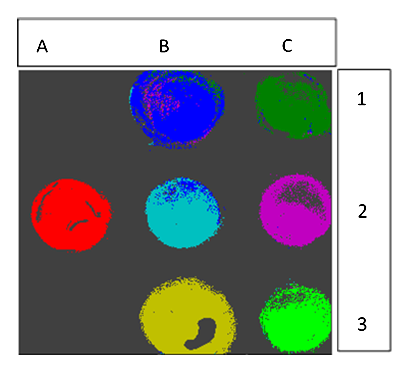
\includegraphics[width=\linewidth]{sample}}
\caption{Badane przetworniki piezoelektryczne.}
\label{fig:sensors}
\end{figure}

Aby dokonać selekcji przetwornika wybrano najprostszy układ geometryczny (patrz: Rys. \ref{fig:sensor_sel_geometry}). Został on wykonany z fragmentu tworzywa sztucznego. Układ oznaczono tak, aby można było ustawić go ponownie w tej samej pozycji po wymianie sensora. Sensor przyklejano na taśmę dwustronną o grubości ok w ustalonym uprzednio miejscu. $1.5mm$. 

\begin{figure}[htbp]
\centering
\fbox{TUTAJ RYSUNEK GEOMETRII CZUJNIKA }%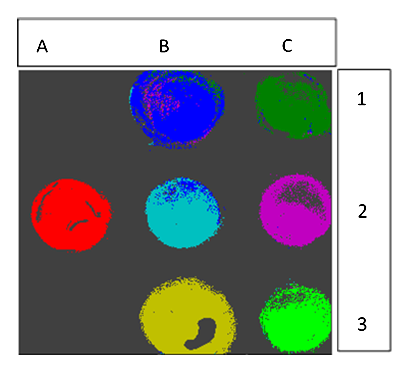
\includegraphics[width=\linewidth]{sample}}
\caption{Konstrukcja pozwalająca na selekcję przetwornika piezoelektrycznego.}
\label{fig:sensor_sel_geometry}
\end{figure}

Dla uzyskania szerszego spektrum danych dla każdego czujniaka powtarzano poamiary w dwóch wariantach: 
\begin{enumerate}
\item stała podpora na jednym z końców układu przetwornika, drugi koniec swobodny,
\item stała podpora na jednym z końców układu przetwornika, drugi koniec z amortyzatorem z gąbki.
\end{enumerate}
Dla każdego pomiaru przeprowadzono po 10 prób, i pozwoliło to zebrać poniższe wyniki. Parametry, jakie wzięto pod uwagę przy ocenie jakości sygnału, to czas trwania ( od inicjalizacji do wygaszenia ) oraz wartość napięcia międzyszczytowego oznaczanych dalej odpowiednio $t_d$ i $V_{pp}$. Ich porównanie po statystycznej analizie przedstawiono na Rys.\ref{fig:sensor_statistic}. Trzeci niebieski słupek w skali od $0\div5$ oznacza subiektywną ocenę poziomu zniekształcenia otrzymanego sygnału. Podczas badań zwracano również uwagę na sposób przyklejenia przetwornika do plastikowego płaskownika tak, aby nie fałszowało to przeprowadzanych pomiarów. 
%TODO Tu przydałby się rozkład widmowy sygnału

\begin{figure}[htbp]
\centering
\fbox{TUTAJ WYKRES PORÓWNAWCZY SYGNAŁÓW }%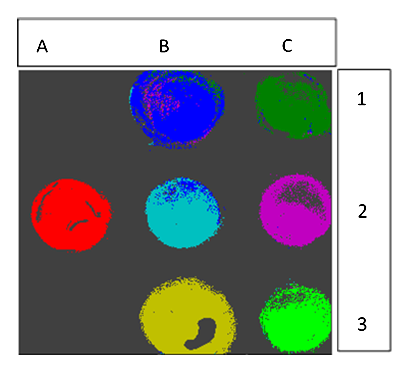
\includegraphics[width=\linewidth]{sample}}
\caption{Zestawienie parametrów sygnałów dla poszczególnych czujników.}
\label{fig:sensor_statistic}
\end{figure}

Na podstawie Rys.\ref{fig:sensor_statistic} możemy stwierdzić, że najwyższą wartość uzyskanego napięcia $V_{pp}$ otrzymaliśmy dla czujnika oznaczonego numerem \textbf{1.2.} Szacuje się, że wyższa wartość $V_{pp}$ będzie bradziej odporna na szumy pochodzące z maszyny, na której sensor byłby umieszczony. Zgodnie z założeniami przeznaczeniem sensora jest przecież licznik impulsów mechanicznych. Z dużym prawdopodobieństwem można uznać, że wyzwalanie licznika następować będzie na jednym ze zboczy pierwszej półfali lub np. wyprostowanej całej fali sygnału. 
\indent Odnośnie czasu trwania sygnału jednoznacznie można stwierdzić, że im krótszy tym lepszy. Pozwala to na wyższą częstotliwość wymuszeń mechanicznych bez wystąpienia zjawiska aliasingu. Oczywiście zbyt krótki, o zbyt małej energii może być problematyczny do wychwycenia - będzie wymagać dużej częstotliwości próbkowania.
\indent Podczas wykonywania pomiarów zauważono ciekawe zaleźności, o których warto wspomnieć przy okazji tego artykułu. Otóż zauważono zależność przebiegu sygnału wyjściowego od rozwiązań konstrukcyjnych zastosowanych w przetworniku. Tak na przykład różnica w zastosowaniu tłumika drgań w postaci gąbki objawia się przede wszystkim czasem trwania sygnału, inaczej mówiąc czasem tłumienia drgań. Jest to wniosek dość oczywisty, jednak warto o nim pamiętać konstruując przetworniki piezoelektryczne. Oprócz tłómików czy filtrów stricte elektrycznych są do dyspozycji również mechaniczne. Gwoli ścisłości w układzie z tłumikiem (patrz: Rys.\ref{fig:scope_with_silencer}) czas wygaszania sgnału wynosi $d_t = TODOs$ i jest krótszy niż w układzie bez tłumika $d_t = TODOs$ (patrz: Rys.\ref{fig:scope_without_silencer}.). Dysproporcja była powtarzalna dla każdego kształtu układu pomiarowego.

\indent Patrząc dalej na te same próbki pomiarów można również dostrzec, że częstotliwość podstawowej harmonicznej sygnału ma bardzo zbliżoną wartość. Nie jest to przypadek. Dzieje się tak ponieważ jest to główna harmoniczna drgań własnych konstrukcji przetwornika. W tym konkretnym przypadku belki o długości $l = mmTODO$ i jednym punkcie mocowania. Projektując przetwornik naleźy zwrócić uwagę, aby odstroić drgania własne konstrukcji od drgań wymuszających. W innym przypadku uzyskamy szum informacyjny. Dalej ma to również wpływ na projektowanie elektronicznego układu przetwornika. W obwodach AC spodziewa się takich właśnie częstotliwości. W następnym akapicie \ref{sec:construction_optymization} mówi się również o zmianie częstotliwości, gdy konstrukcja jest belką o dwóch punktach podparcia. 

Napięcie $V_{pp}$ wykazuje się niezmiennością w odniesieniu do przedstawionych zmian w konstrukcji. Jednak jest ono zależne od zupełnie innego parametru, od energii zderzenia. Jest ona bezpośrednią przyczyną ugięcia belki z przetwornikiem. Energia zderzenia, a dokładniej ta stracona, oraz czas kontaktu z belką stanowią ważne parametry dla przebiegu sygnału napięciowego przetwornika. Więcej na ten temat w akapicie \ref{sec:construction_optymization}.

\begin{figure}[htbp]
\centering
\fbox{PRZEBIEG DLA PRÓBKI 1.2. }%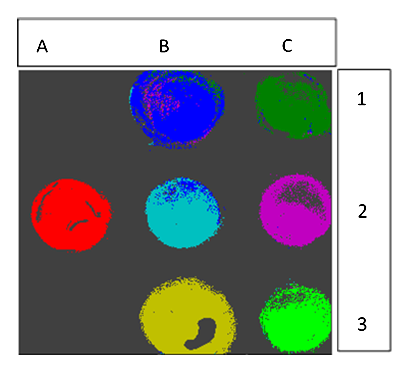
\includegraphics[width=\linewidth]{sample}}
\caption{Przykładowy przebieg pojedynczego sygnału dla próbki oznaczonej roboczo 1.2Acs15dt.}
\label{fig:scope_without_silencer}
\end{figure}

\begin{figure}[htbp]
\centering
\fbox{PRZEBIEG DLA PRÓBKI 1.2. }%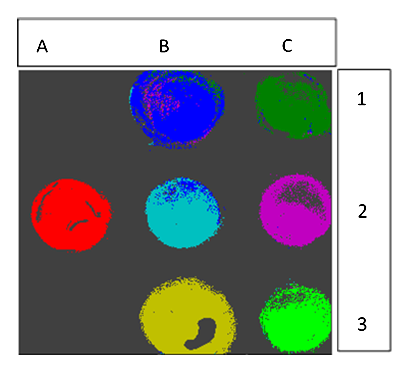
\includegraphics[width=\linewidth]{sample}}
\caption{Przykładowy przebieg pojedynczego sygnału dla próbki oznaczonej roboczo 1.2Acf15dt.}
\label{fig:scope_with_silencer}
\end{figure}
